% =================================================================================================
% File:			gestione_contenuti.tex
% Description:	Definisce la sezione relativa ad un capitolo del documento
% Created:		2015-04-25
% Author:		Santacatterina Luca
% Email:		santacatterina.luca@mashup-unipd.it
% =================================================================================================
% Modification History:
% Version		Modifier Date		Change											Author
% 0.0.1 		2015-05-245			inizio stesura sezione capitolo					Santacatterina Luca
% =================================================================================================
%

% CONTENUTO DEL CAPITOLO

\section{Gestione contenuti} % (fold)
\label{sec:gestione_contenuti}
	Dopo aver eseguito le istruzioni per l'autenticazione\gloss{} viene visualizzata la dashboard\gloss{} dell’applicazione.\newline
	Nella schermata principale della dashboard\gloss{} vengono visualizzati in riquadri le \textbf{recipes}\gloss{} disponibili nel sistema (Figura: \ref{fig:ricette_disponibili}), mentre nella sinistra dell'applicazione è disponibile il menù principale di gestione (Figura: \ref{fig:menu_principale_utente})
	\begin{figure}[H]
		\centering
		\centerline{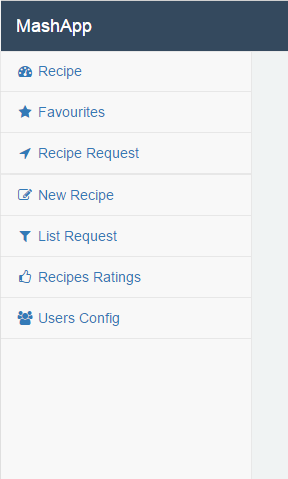
\includegraphics[width=6cm]{images/menu_principale_amministratore.png}}
		\caption{Menù principale amministratore}
		\label{fig:menu_principale_utente}
	\end{figure}

% section Gestione contenuti (end)